\chapter{Experiments and Results}
\label{chapter:experiments}

This chapter summarizes the experiments carried out for our proposed model, the Softmax Mixture, and several pointer based models. We also discuss the results obtained when applying these models on the LAMBADA dataset.

All the experiments described in this chapter have been implemented using Tensorflow v1.4 \cite{tensorflow2015}. The code is publicly available at \url{https://github.com/moisestg/rare-lm}.

\section{Softmax Mixture Model}

\subsection{Experimental Setup}

The original LAMBADA dataset contains lowercased text. As will be described in the upcoming experiments section, part of our preprocessing requires PoS tagging the text. Although there are caseless PoS taggers available, in order to maximize the accuracy of this step we opted to use the capitalized version of the dataset\footnote{Available at \url{http://clic.cimec.unitn.it/lambada/train-novels-capitalized.txt.gz}}.

Additionally, we delimited each novel in the corpus with a special a tag and used that to randomize the order in which the novels are fed to the model for each epoch.

Furthermore, following the recommendations from \cite{merity2016pointer} we modified our base code resulting in a much faster implementation: During the training phase it is only necessary to compute the softmax probability of the target word (rather than the whole vocabulary) in order to compute the cross-entropy loss, as the observed distribution is a one-hot encoding of the correct output.

Finally, \autoref{trainSmm} summarizes the specific training configuration used in the following set of experiments:

\begin{table}[]
	\centering
\begin{tabular}{|c|c|}
	\hline
	\textbf{Training data}                                                     & 1/3 of all the training novels                                                              \\ \hline
	\textbf{Development data}                                                  & \begin{tabular}[c]{@{}c@{}}100K contiguous sentences\\  from the remaining 2/3\end{tabular} \\ \hline
	\textbf{Vocabulary size}                                                   & 44636                                                                                       \\ \hline
	\textbf{Word embeddings}                                                   & \begin{tabular}[c]{@{}c@{}}150-d word2vec (pretrained\\ on the training data)\end{tabular}  \\ \hline
	\textbf{Optimizer}                                                         & \begin{tabular}[c]{@{}c@{}}ADAM with learning \\ rate of 0.001 \end{tabular}             \\ \hline
	\textbf{TBPPT}                                                             & $k_1=1$ and $k_2=20$                                                                        \\ \hline
	\textbf{Batch size}                                                        & 64                                                                                          \\ \hline
	\textbf{\begin{tabular}[c]{@{}c@{}}Maximum global \\ L2 norm\end{tabular}} & 8                                                                                           \\ \hline
	\textbf{Training epochs}                                                     & 10 \\ \hline
\end{tabular}
	\caption{Training configuration for \autoref{sec:smmExps}.}
	\label{trainSmm}
\end{table}

\subsection{Experiments}
\label{sec:smmExps}

As described in \autoref{sec:mixtureModel}, the Softmax Mixture model has the ability to encode two differentiated output distributions that are dynamically blended by the switching network. In order to train the switching component in a supervised fashion, we need to tag each word in the training set with its corresponding source. 

Motivated by our preliminary analysis of LAMBADA, we decided to tag peoples' names as they are a very specific subset of rare words that a vanilla softmax output layer fails to handle. By using a predefined list\footnote{Available at \url{https://deron.meranda.us/data/}.}, we also made sure to reduce the amount of false positives (at the expense of missing some rare or fictitious names).

In our first batch of experiments we started exploring the space of hyperparameters by finding an optimal value for $\lambda$, the weight of the loss term in charge of the training supervision of the switching component. \autoref{fig:lambdaPerplexity} shows the evolution of the development perplexity during training for the explored range of values. We can see that values of $\lambda$ up to 100 produce a similar behavior on the overall perplexity of the model. Higher values start to noticeably hinder the learning process as the sigmoid loss of the switching component starts to overcome the cross-entropy loss.

\begin{figure}[H]
	\centering
	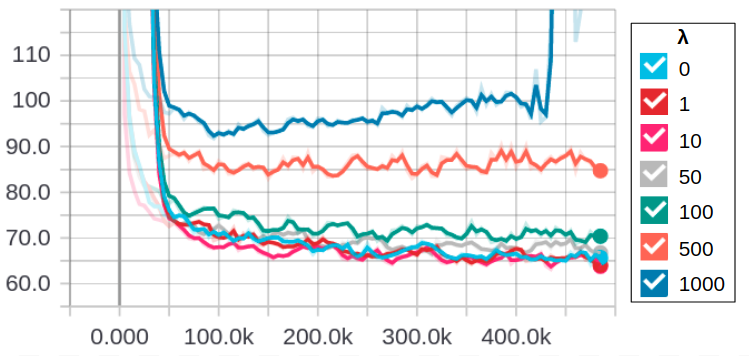
\includegraphics[scale=0.4]{lambdaPerplexity}
	\captionof{figure}{Development perplexity traces for different values of lambda.}
	\label{fig:lambdaPerplexity}
\end{figure}

\begin{table}[H]
	\centering
	\makebox[\textwidth][c]{\begin{tabular}{cc|c|c|c|c|}
		\cline{3-6}
		\multicolumn{1}{l}{}                                                    & \multicolumn{1}{l|}{}   & \multicolumn{2}{c|}{\textbf{All words}} & \multicolumn{2}{c|}{\textbf{Names}} \\ \cline{3-6} 
		&                         & \textbf{Train}       & \textbf{Dev}        & \textbf{Train}        & \textbf{Dev}         \\ \hline
		\multicolumn{1}{|c|}{\multirow{2}{*}{\textbf{No regularization}}}                            & \textbf{\textbf{Baseline}}                & 42.5        & 61.5       & 1000         & 130K        \\ \cline{2-6} 
		\multicolumn{1}{|c|}{}                                                  & \textbf{Mixture ($\boldsymbol{\lambda}\mathbf{=100}$)} & 55          & 69         & 4000         & 120K        \\ \hline
		\multicolumn{1}{|c|}{\multirow{2}{*}{\textbf{Input dropout}}}                    & \textbf{Baseline}                & 52.5        & 63         & 2000         & 140K        \\ \cline{2-6} 
		\multicolumn{1}{|c|}{}                                                  & \textbf{Mixture ($\boldsymbol{\lambda}\mathbf{=100}$)} & 65          & 72         & 8000         & 120K        \\ \hline
		\multicolumn{1}{|c|}{\multirow{2}{*}{\textbf{State dropout}}}                    & \textbf{Baseline}                & 48          & 62.5       & 1000         & 120K        \\ \cline{2-6} 
		\multicolumn{1}{|c|}{}                                                  & \textbf{Mixture ($\boldsymbol{\lambda}\mathbf{=100}$)} & 62.5        & 73         & 6000         & 120K        \\ \hline
		\multicolumn{1}{|c|}{\multirow{2}{*}{\textbf{Output dropout}}}                   & \textbf{Baseline}                & 62.5        & 65         & 5000         & 150K        \\ \cline{2-6} 
		\multicolumn{1}{|c|}{}                                                  & \textbf{Mixture ($\boldsymbol{\lambda}\mathbf{=100}$)} & 80          & 73         & 20K          & 80K         \\ \hline
		\multicolumn{1}{|c|}{\multirow{2}{*}{\textbf{L2 regularization ($\boldsymbol{\beta}\mathbf{=0.01}$)}}} & \textbf{Baseline}                & 100         & 125        & 10K          & 400K        \\ \cline{2-6} 
		\multicolumn{1}{|c|}{}                                                  & \textbf{Mixture ($\boldsymbol{\lambda}\mathbf{=100}$)} & 107.5       & 119        & 8000         & 120K        \\ \hline
	\end{tabular}}
	\caption{Perplexity for different regularization techniques.}
	\label{smmExps}
\end{table}

\begin{figure}[H]
	\centering
	\makebox[\textwidth][c]{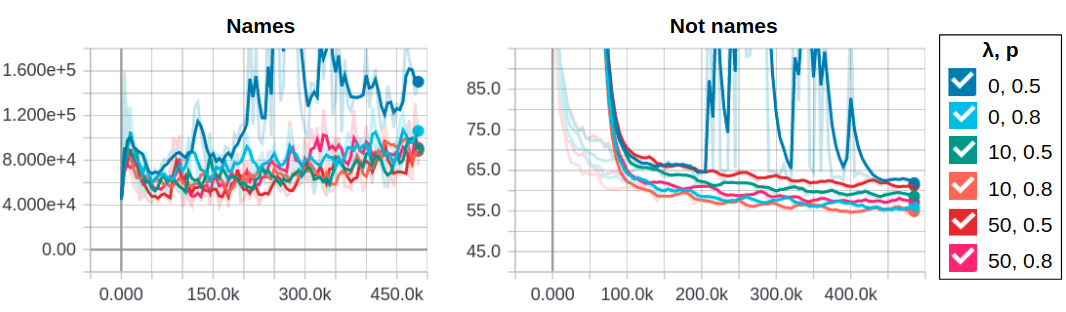
\includegraphics[scale=0.425]{outDropPerplexities}}
	\captionof{figure}{Development perplexity traces for different combinations of lambda and output keep probability.}
	\label{fig:outDropPerplexities}
\end{figure}

\begin{table}[H]
	\centering
	\begin{tabular}{cc|c|c|}
		\cline{3-4}
		&                                                                                                               & \textbf{Names} & \textbf{Not names} \\ \hline
		\multicolumn{1}{|c|}{\multirow{3}{*}{$\boldsymbol{\lambda}\mathbf{=10}$}} & $\mathbf{p=0.5}$                                                                                              & 62K            & 59                 \\ \cline{2-4} 
		\multicolumn{1}{|c|}{}                                                    & $\mathbf{p=0.8}$                                                                                              & 65K            & 54                 \\ \cline{2-4} 
		\multicolumn{1}{|c|}{}                                                    & \begin{tabular}[c]{@{}c@{}}$\mathbf{p_{\text{names}}=0.5}$\\ $\mathbf{p_{\text{not names}}=0.8}$\end{tabular} & 55K            & 54                 \\ \hline
		\multicolumn{1}{|c|}{\multirow{3}{*}{$\boldsymbol{\lambda}\mathbf{=50}$}} & $\mathbf{p=0.5}$                                                                                              & 53K            & 61                 \\ \cline{2-4} 
		\multicolumn{1}{|c|}{}                                                    & $\mathbf{p=0.8}$                                                                                              & 58K            & 57                 \\ \cline{2-4} 
		\multicolumn{1}{|c|}{}                                                    & \begin{tabular}[c]{@{}c@{}}$\mathbf{p_{\text{names}}=0.5}$\\ $\mathbf{p_{\text{not names}}=0.8}$\end{tabular} & 52K            & 57                 \\ \hline
	\end{tabular}
	\caption{Development perplexity comparison between regular and ``splitted'' dropout.}
	\label{splittedDropPerplexities}
\end{table}

Study classifier in isolation, confussion matrix, examples of predictions (qualitatively)! 3\% of names out af all words  

\begin{table}[H]
	\centering
	\begin{tabular}{cc|c|c|}
		\cline{3-4}
		&                   & \multicolumn{2}{c|}{\textbf{Prediction}} \\ \cline{3-4} 
		&                   & \textbf{Name}     & \textbf{Not name}    \\ \hline
		\multicolumn{1}{|c|}{\multirow{2}{*}{\textbf{\begin{tabular}[c]{@{}c@{}}Ground\\ Truth\end{tabular}}}} & \textbf{Name}     & 20859             & 20292                \\ \cline{2-4} 
		\multicolumn{1}{|c|}{}                                                                                 & \textbf{Not name} & 123220            & 1874029              \\ \hline
	\end{tabular}
	\caption{Confusion matrix for name classifier.}
	\label{confMatrix}
\end{table}

\begin{table}[H]
	\centering
	\begin{tabular}{c|c|c|}
		\cline{2-3}
		& \textbf{Names}        & \textbf{All words}  \\ \hline
		\multicolumn{1}{|c|}{\multirow{3}{*}{\textbf{Ground truth}}}                                                                & \multirow{3}{*}{5K} & \multirow{3}{*}{57} \\
		\multicolumn{1}{|c|}{}                                                                                                      &                       &                     \\
		\multicolumn{1}{|c|}{}                                                                                                      &                       &                     \\ \hline
		\multicolumn{1}{|c|}{\multirow{3}{*}{\textbf{\begin{tabular}[c]{@{}c@{}}Ground truth and\\ splitted dropout\end{tabular}}}} & \multirow{3}{*}{4K} & \multirow{3}{*}{55} \\
		\multicolumn{1}{|c|}{}                                                                                                      &                       &                     \\
		\multicolumn{1}{|c|}{}                                                                                                      &                       &                     \\ \hline
	\end{tabular}
	\caption{Perplexity with ground truth switching.}
	\label{groundTruthPerplexities}
\end{table}

\begin{table}[H]
	\centering
	\begin{tabular}{|c|c|c|c|}
		\hline
		Lily & Rachel & England & English \\ \hline
		\makecell{Dean\\Xavier\\David\\Lily\\Noah\\Al\\Alex\\Hunter\\Eric\\Derek} & \makecell{Caroline\\Hunter\\Elizabeth\\Emma\\David\\Julia\\Trevor\\Zoe\\Dan\\Kim} & \makecell{London\\America\\England\\Santa\\Paris\\France\\Little\\North\\Paul\\English} & \makecell{English\\French\\Christian\\Irish\\German\\Roman\\Marine\\Fae\\Dean\\Sunday} \\ \hline
	\end{tabular}
	\caption{Top 10 predictions for words tagged as names.}
	\label{my-label}
\end{table}

JSD of 0.69 (maximum) vs 0.2?

Make te case for using nouns rather names and also explain why not proper nouns (very few too). Include something about names?-> Say that now classification task is easier but however no overall improvements are observed?

\section{Pointer Based Models}
\label{sec:pointerExps}

\subsection{Experimental Setup}

\subsection{Experiments}

Start reasoning global vs local?

When showing the PSMM mention the initialization of $\mathbf{s}$ and the issue with the gradient.

\begin{table}[H]
	\centering
	\begin{tabular}{c|c|c|}
		\cline{2-3}
		\multicolumn{1}{l|}{}                            & \textbf{Control} & \textbf{LAMBADA} \\ \hline
		\multicolumn{1}{|c|}{\textbf{LSTM-512}}          & 149              & 5357             \\ \hline
		\multicolumn{1}{|c|}{\textbf{Continuous Cache}}               & 129              & 138              \\ \hline
		\multicolumn{1}{|c|}{\textbf{PSMM (length=100)}} & 114              & 154              \\ \hline
		\multicolumn{1}{|c|}{\textbf{PSMM (length=200)}} & 116              & 172              \\ \hline
	\end{tabular}
	\caption{Perplexity.}
	\label{psmmExps}
\end{table}

\begin{figure}[H]
	\centering
	\makebox[\textwidth][c]{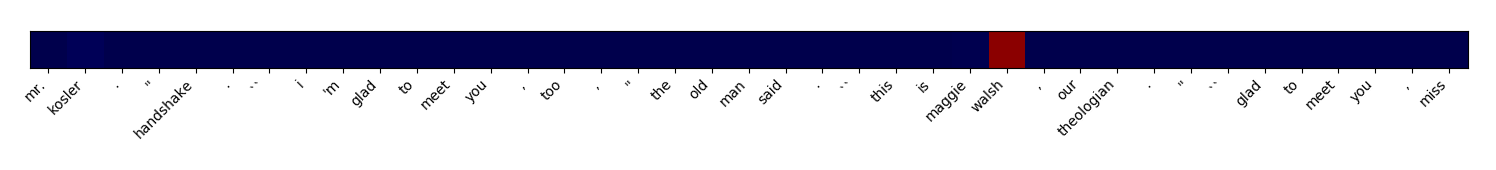
\includegraphics[scale=0.305]{gatesEx2}}
	\captionof{figure}{Predicting ``walsh'' ($g_t=0.07$).}
	\label{fig:gateEx2}
\end{figure}

\begin{figure}[H]
	\centering
	\makebox[\textwidth][c]{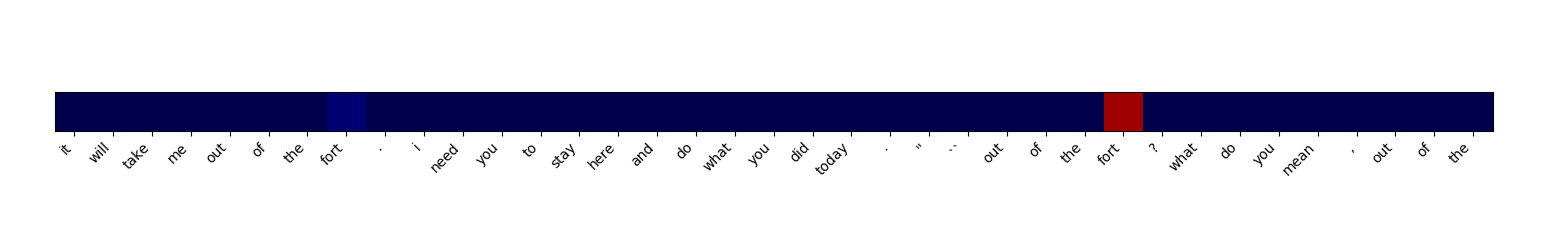
\includegraphics[scale=0.3]{gateEx1}}
	\captionof{figure}{Predicting ``fort'' ($g_t=0.28$).}
	\label{fig:gateEx1}
\end{figure}

\begin{figure}[H]
	\centering
	\makebox[\textwidth][c]{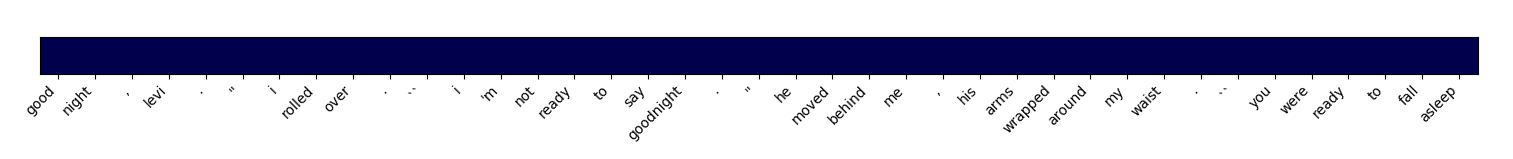
\includegraphics[scale=0.3]{gateEx3}}
	\captionof{figure}{Predicting ``earlier'' ($g_t=0.99$).}
	\label{fig:gateEx3}
\end{figure}